\documentclass[10pt]{extarticle}
\usepackage[paperwidth=7.07in,paperheight=9.43in,margin=0.95in]{geometry}
\usepackage{fontspec}
\setmainfont{Latin Modern Roman}
\setmonofont{Menlo}[Scale=0.85]
\usepackage{amsmath,amssymb}
\usepackage{booktabs,tabularx}
\usepackage{enumitem}
\usepackage{microtype}
\usepackage{tikz}
\usetikzlibrary{arrows.meta,positioning,calc,fit}
\tikzset{>=Stealth}
\tikzset{every picture/.append style={line width=0.6pt,font=\footnotesize}}
\usepackage[hidelinks]{hyperref}
\usepackage{parskip}
\usepackage{ragged2e}
\linespread{1.08}
\RaggedRight
\setlength{\emergencystretch}{3em}
\pagestyle{plain}
\setlist{topsep=0.3em,itemsep=0.3em,parsep=0pt}
\renewcommand{\arraystretch}{1.25}
\newcolumntype{Y}{>{\RaggedRight\arraybackslash}X}

\newcommand{\you}[2]{{\small[\textbf{you}, #1: \textit{``#2''}]}}
\newcommand{\youx}[1]{{\small[\textbf{you}, #1]}}
\newcommand{\agreed}[1]{{\small[\textbf{agreed} #1]}}
\newcommand{\prop}{{\small[\textbf{proposal}]}}
\newcommand{\open}[1]{\par\noindent\fbox{\parbox{\dimexpr\linewidth-2\fboxsep-2\fboxrule}{\textbf{Open.} #1}}\par}
\newcommand{\Sec}[1]{\section*{#1}\addcontentsline{toc}{section}{#1}}
\newcommand{\Sub}[1]{\subsection*{#1}}
\newfontfamily\nerd{JetBrainsMonoNerdFont-Regular.ttf}[Path=/Users/alecmitchell-thomson/Library/Fonts/,Renderer=HarfBuzz]
\newcommand{\g}[1]{{\nerd\char"#1}}

\begin{document}

{\Large\bfseries Locus plan}\\[0.3em]
{\small Version 4, 19 October 2026: final. Everything settled between 14 and 19 October, including your markups of versions 2 and 3 and the screens. Companion: \textit{Locus: information and links} (\texttt{info.tex}). The screens are settled from here in the ratatui prototype, not on paper.}

\medskip
\noindent\fbox{\parbox{\dimexpr\linewidth-2\fboxsep-2\fboxrule}{%
\textbf{What your version 3 markup changed}
\begin{itemize}[leftmargin=1.2em]
\item \textbf{Information has three kinds}, sources, work and learning state, each with one area label; the library of sources only grows, by design (C.2 and the companion).
\item \textbf{Links join ideas, decisions and concepts}, judged by Claude with a reason; the old engine keeps reading and search, and its word links are retired (C.4).
\item Interview prep is part of the learning system; the CV is a light Careers project; chores are offered while you wait on Claude; search jumps to the source; ink reads curly brackets; the desktop leaves the plan.
\end{itemize}
Changes carry the date 19 October.}}

\Sec{How to read and mark this}

Every decision carries a tag saying where it came from:
\begin{itemize}
\item \you{date}{quote}: your words in our conversation.
\item \agreed{date}: I proposed it, you accepted it.
\item \prop: my suggestion, not yet discussed. Look at these hardest.
\end{itemize}

This version is for a final read before building starts. What is still open sits in Part~G. As before: a circled \textbf{?} for anything to explain, a circled \textbf{\texttimes} for anything wrong, a strike-through for something you have changed your mind on. Draw arrows from a note to the text it is about.

\tableofcontents

\clearpage
\Sec{A. The goal and the rules}

\Sub{The goal}
\you{16 Oct}{make this something I actually use and find useful, and is intelligent and makes me better, not something annoying that I avoid and drop after a while.} Every corner of the plan is to be settled before building, with each decision traceable to this conversation \youx{16 Oct}.

\textbf{North star.} \you{14 Oct}{to make it as frictionless as possible all to enable me to work on effectively, learn and understand my projects and work as quickly and as deeply as possible.} Claude does most of the building; locus exists so that you stay the person who understands what is being built and why, well enough to \you{14 Oct}{come up with ideas, question decisions claude made, and be able to propose fixes/ new directions.}

\Sub{The evidence from the old locus}
Measured on the server, 16 October:
\begin{itemize}
\item \textbf{Used and still used:} tablet ink capture (431 marks, still running); pushing documents to the tablet; reading ink back. The QUAST dossier drew about 60 marks in half an hour.
\item \textbf{Built and abandoned:} 77 daily pages pushed, 6 read back, the last on 7 August. No recall card ever graded. Margin answers and keep/reject verdicts stop in early August.
\item \textbf{Built and never used:} corpus search was called once through the MCP; \texttt{critique} and \texttt{synthesise} never.
\item \textbf{Fragile:} the MCP started 2,325 processes to serve 75 calls; rmapi had a 12-day outage in August; repositories have not been re-ingested since June; reading discovery accepted 4 of 2,571 candidates.
\end{itemize}
The pattern: work that reached you on paper, about a project you were in, got used. Work that arrived unasked, on a schedule, about things you were not doing, did not.

\Sub{The rules every feature is judged by}
\begin{enumerate}[label=R\arabic*.]
\item \textbf{Every feature is one you would miss.} \you{14 Oct}{I want to keep noise and clutter to an absolute minimum.}
\item \textbf{Only what you are working on now.} \you{14 Oct}{I mostly only care about the projects that I am working on now.}
\item \textbf{Bad output is worse than none.} If something cannot be good, it does not ship.
\item \textbf{Ease first, depth once fluent.} \you{16 Oct}{ease and ability first for adoption, then later once I am a fluent user we can add more complex behaviour.}
\item \textbf{Reliability is a feature.} Anything that disconnects or lags gets abandoned.
\item \textbf{Links must do real work,} and each one says why it matters (Part~C.4).
\item \textbf{Each surface has one job.} Paper is for understanding. The locus window is where you check and act. The project window is where you work.
\item \textbf{Nothing interrupts you uninvited.} \agreed{16 Oct} Not even a status-line hint \youx{17 Oct}.
\item \textbf{Every feature is reviewed on use.} Each logs its use; unused features come up in the weekly review to fix or cut \agreed{16 Oct}.
\item \textbf{Never stale.} \you{16 Oct}{Never want locus to confront me with a stale/out of date decision.} Anything not yet checked against recent work says so.
\item \textbf{Looks matter.} \you{18 Oct}{I want to be excited to have it on the side of my screen}; a bad-looking TUI is \you{18 Oct}{another reason the system does not get adopted by me.}
\end{enumerate}

\clearpage
\Sec{B. The system}

\Sub{B.1 Apps and names}
\begin{itemize}
\item \textbf{locus} is the whole system, its repository and its window \youx{14 Oct}.
\item \textbf{heuris} is the knowledge app: \you{18 Oct}{to find/ discover/ invent - pretty apt and looks/ sounds good}. It replaces the name nous.
\item \textbf{kairos} (time) and \textbf{keryx} (mail) are the existing Rust apps, each a terminal UI over its own daemon.
\item \textbf{aulos} leaves: \you{16 Oct}{aulos is just music, it can stay separate.}
\item \textbf{chores} are short things you tend to put off, offered in a gap, including while you wait on Claude: \you{19 Oct}{gap could be waiting for claude, just a small amount of time}. (Your word.) \textbf{scout} is heuris's background agent \youx{18 Oct}; \textbf{Explore} and \textbf{Jot} keep their names.
\item The repositories merge into one later, once the shared root has real contents \agreed{16 Oct}.
\item All of it is one system: \you{19 Oct}{all linked together to form one system that knows about everything.}
\end{itemize}

\Sub{B.2 Who owns what}
Each object has one owning app, and only the owner writes it; the others display it and send requests to the owner \agreed{17 Oct}.

\begin{tabularx}{\linewidth}{@{}l l Y@{}}
\toprule
Object & Owner & Others \\
\midrule
Events, work blocks & kairos & Home links to the day in Calendar \\
Tasks and chores & kairos & Home shows the slice that fits now; done and snooze go to kairos \youx{17 Oct} \\
Deadlines & kairos & keryx and Canvas propose; you approve \\
Mail & keryx & a task made from mail links back to its thread \\
Dossiers, answers, Explore, interview prep & heuris & Project view and Home show them \youx{17 Oct} \\
Background jobs & locus core & Home and System show them \\
Areas, streams, repository registry & shared root & every app reads them \\
Notes repository & you & locus writes only with your approval: filed jots, exported ink \youx{19 Oct} \\
\bottomrule
\end{tabularx}

\Sub{B.3 Taxonomy}
Unchanged from 15 October except for names. Areas: Studies, Projects, Careers, Personal. Streams under each. Shape is inferred: \textbf{event}, \textbf{work} or \textbf{chore}; a deadline is an attribute, hard or soft, owed or self-chosen.

kairos moves to the shared taxonomy in Slice 0: \you{17 Oct}{Migrating kairos is absolutely fine, just remember I want the filter granularity of streams within family but not the other areas.} So Personal filters by stream (Family, Sport, Social, Travel with Errands); Studies, Projects and Careers filter as whole areas. (``Family'' read as Personal; left unmarked in version 2, so taken as right.)

\Sub{B.4 Where you meet it}
\textbf{Your screens} \youx{17 Oct}. On the ultrawide: the right two-thirds is the project window (Claude chats, nvim); the left third is two stacked windows, locus above and aulos below, each about 95 by 38 characters.

The desktop itself (AeroSpace, the workspace bar) is set up and tested on both screens, and sits outside locus: \you{19 Oct}{not relevant to locus}. On the laptop, locus has its own workspace rather than the quick terminal.

\textbf{The locus window} runs a tmux session called \texttt{locus} with one window per view \youx{17 Oct}; your locus project session is now \texttt{locus-dev}. Views are switched with \texttt{Alt-1} to \texttt{Alt-4}, since kairos uses the bare digits for its filters:

\begin{tabularx}{\linewidth}{@{}l l Y@{}}
\toprule
Key & View & \\
\midrule
\texttt{Alt-1} & Home & everything at a glance \\
\texttt{Alt-2} & Project & the project your project window is on \\
\texttt{Alt-3} & Calendar & kairos \\
\texttt{Alt-4} & Mail & keryx \\
\bottomrule
\end{tabularx}

\textbf{The Project view follows you.} A tmux hook tells it which session your project window switched to \you{17 Oct}{I like the idea of the 3 views with the project view automatically switching to whatever project I am focussed on in the main window.} It never moves you between views, never switches while you are scrolling or typing in it, and \texttt{m} pins it. No popup: \you{16 Oct}{not sure I feel a popup would ever be kept.}

\textbf{The phone} only shows the synced iCloud calendar. The kairos approve buttons and the ntfy pushes are switched off: \you{16 Oct}{the accept/reject kairos and check-up ntfy pushes were just noise.}

\Sub{B.5 Working mode}
One project per deep block, two or three projects a week: \you{18 Oct}{most weeks I will not want to entirely focus on just one project, probably deep focus blocks for two or even three.} Other projects run only if they can be left: \you{18 Oct}{I do not want to often be switching to other ones, unless they are ones that are fine being left unattended.} The \textbf{attended} project is the one in the current kairos work block, or the one you mark with \texttt{m}.

\Sub{B.6 How it is built and run}
\you{16 Oct}{code written locally, then pushed to server and run there for services/always running jobs (like other projects (kairos))}. One long-lived HTTP service on the server, over Tailscale with a token, replaces the one-process-per-chat MCP. Background work runs headless with \texttt{claude -p} \youx{14 Oct}.

\clearpage
\Sec{C. heuris}

\Sub{C.1 What it does}
\begin{enumerate}
\item \textbf{Dossiers.} Each project's understanding, built from its repositories and chats, kept current.
\item \textbf{Answers.} Questions from the ask line, and circled \textbf{?} marks on paper, answered and linked to the passage.
\item \textbf{Learning documents and readback.} Explainers on the tablet; your ink read back and sorted into answers, decisions and format feedback.
\item \textbf{Explore and the scout.} An idea board for your projects and new ones: \you{17 Oct}{a sort of idea generator for my current projects/ new projects.}
\item \textbf{Context for working chats.} Each project's CLAUDE.md points at its decision log and dossier \agreed{16 Oct}; every area of your life gets a brief any chat can read (C.13).
\item \textbf{The learning system.} Goals you set, tracked and guided through to understanding: \you{19 Oct}{my own personal course-generator that knows what I am already good at}. Interview prep is a part of it (C.10, C.11).
\end{enumerate}

\Sub{C.2 Where its knowledge comes from}
Everything is one of three kinds, \textbf{sources} (to read; each rarely changes, but there are always more), \textbf{work} (in motion) and \textbf{learning state} (facts about you), and carries one area label. The companion document sets out what each kind means for what sees it \youx{19 Oct}. The library of sources only grows, and that is a design requirement: \you{19 Oct}{the library of sources is ever expanding as I accumulate more, that should be a key design feature.} Arrival is automatic, each new source costs a fixed amount and is labelled and linked on arrival, search moves to an index as it grows, and nothing is pruned.


Each kind of source is stored by how fast it changes \you{17 Oct}{I like C as described, it seems like the best framework for how I work.}

\begin{figure}[h]
\centering
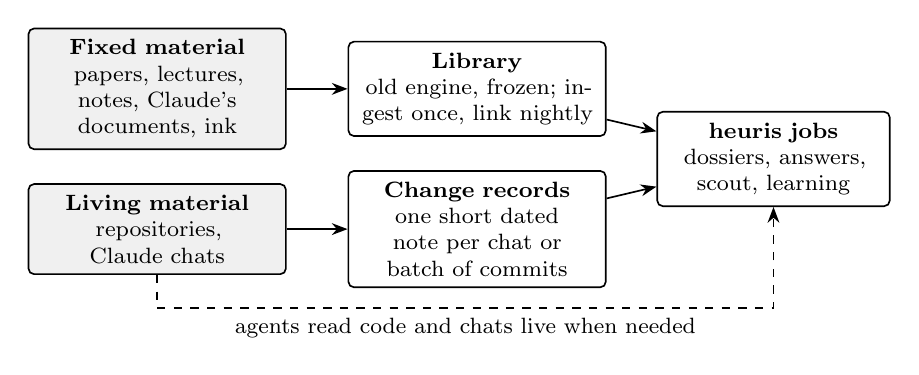
\begin{tikzpicture}[
  box/.style={draw,rounded corners=2pt,align=center,inner sep=4pt,text width=8.5em},
  src/.style={box,fill=black!6}]
\node[src] (fixed) {\textbf{Fixed material}\\papers, lectures, notes, Claude's documents, ink};
\node[src,below=1.2em of fixed] (living) {\textbf{Living material}\\repositories, Claude chats};
\node[box,right=2.2em of fixed] (lib) {\textbf{Library}\\old engine, frozen; ingest once, link nightly};
\node[box,right=2.2em of living] (rec) {\textbf{Change records}\\one short dated note per chat or batch of commits};
\node[box,anchor=west,text width=7.6em] (jobs) at ($(lib.east)!0.5!(rec.east)+(1.8em,0)$) {\textbf{heuris jobs}\\dossiers, answers, scout, learning};
\draw[->] (fixed) -- (lib);
\draw[->] (living) -- (rec);
\draw[->] (lib) -- (jobs);
\draw[->] (rec) -- (jobs);
\draw[->,dashed] (living.south) |- ++(0,-1.2em) -| node[pos=0.25,below]{agents read code and chats live when needed} (jobs.south);
\end{tikzpicture}
\end{figure}

\begin{itemize}
\item \textbf{The library} keeps what the old engine does well: faithful reading of PDFs with maths and figures into searchable text. Its nightly word-matching links are retired (C.4). It is frozen: fixes, no features. The nightly chain shrinks from 12 steps to ingest, link, back up.
\item \textbf{Its state, checked 19 October,} after you asked \you{19 Oct}{does the old engine still work?}: 242 documents, the nightly jobs all succeed, but \textbf{nothing has been added since 6 September}. The nightly links are weak: they join documents through generic words such as ``regime'', ``Trade'' or ``Order''. A filter for such words is already built and switched off. Slice 0 finds why nothing is arriving (the likely cause: no file watcher runs on the server; four papers dropped on 31 July are still waiting). Links are then rebuilt on meaning, not words (C.4): \you{19 Oct}{evaluate what is actually useful content}.
\item \textbf{Change records.} When a Claude chat ends, or new commits reach the server, a small job reads only what is new and writes what changed, what was decided (your words quoted), results, open questions and which dossier sections it touches. This is how R10 holds without rebuilding everything \agreed{17 Oct}.
\item \textbf{Questions across projects} go to an agent that searches your other repositories and chats on demand \youx{16 Oct}. One use you named: \you{19 Oct}{useful for writing my CV - describing projects}.
\item \textbf{Search} gets a plain full-text index over chats and change records, so \texttt{/} covers everything \youx{18 Oct}. Enter on a result jumps to it where it lives: the chat at that moment, the note in nvim at that line, the PDF at that page, the decision in Decisions \you{19 Oct}{need to be able to jump to whatever search returns to read in context}. Its use is logged so we learn what it is for: \you{19 Oct}{need to monitor how I would actually use it/what for}.
\item Laptop transcripts sync to the server. Transcript retention is now ten years on both machines (it defaulted to 30 days); done 18 October.
\end{itemize}

\Sub{C.3 What happens to the old locus}
\begin{tabularx}{\linewidth}{@{}l Y@{}}
\toprule
Keep & library engine (frozen) for reading and search, ink capture, tablet push (after fixes), evaluation, backups (trimmed from 20\,GB) \\
Restructure & repository sync and chat capture into change records; the connection writer into dossier links; margin answers into Answered; discovery into the scout; the MCP into one service \\
Remove & nightly word-matching links, daily page and its readback, recall, contradiction tracker, Obsidian export, \texttt{critique}/\texttt{synthesise}, repository ingest, and their nightly steps \\
\bottomrule
\end{tabularx}

\Sub{C.4 Links}
The old links joined documents that shared a word. Your fix: \you{19 Oct}{links are more than just words - they should be ideas/decisions/concepts.} A link joins two units of meaning, an idea, a decision or a concept, across all three kinds of information, including between sources, work and Explore \youx{19 Oct}.
\begin{itemize}
\item \textbf{The linking job:} candidates come cheaply from anything new (a change record, a new source, an Explore idea), matched by meaning and shared concepts; Claude keeps a pair only if it can write the one sentence saying why it matters to you \prop.
\item \textbf{Shown in place only}: inside a dossier beside the decision, an answer, a scout find, one of your Explore ideas. No graph or daily page of links \agreed{17 Oct}. Most valuable where \you{19 Oct}{scout comes up with ideas linking my projects externally or linking them together.}
\item \textbf{Later}: your decision network, \you{19 Oct}{decision network/graph would be interesting to view}, grows out of this in the research track.
\end{itemize}

\Sub{C.5 Ink, and where each mark points}
\you{18 Oct}{comments linking to the wrong part end up meaning almost absolutely nothing.} You often draw an arrow from a note to its text \youx{18 Oct}.
\begin{itemize}
\item On Claude's documents, LaTeX's position map (SyncTeX) and hidden block IDs turn a mark's position into the exact paragraph or decision. On other PDFs, the position of every word does the same job. A cropped image of the mark and its candidate text is then checked by Claude, which follows arrows and brackets, including your curly brackets: \you{19 Oct}{I also draw curly brackets over the part of a passage that my note refers to, with the point of the bracket often pointing to my note.}
\item When unsure, it asks in the approve list. Enter shows a crop of your mark beside two or three numbered passages it might point at; you press the number, or \texttt{x} for ``a general note'' \agreed{19 Oct}.
\item \textbf{Highlighter marks are read too.} Version 2's readback missed one: the tablet stores the exact highlighted text, which locus ignored. Fixing it makes a highlight the one mark that is always placed correctly.
\item \textbf{Gate:} at least 95\% placed correctly on your QUAST, brief v1 and v2 markups before anything is built on ink \youx{18 Oct}.
\item \textbf{Every reading document} has an even margin on all four sides: \you{18 Oct}{things on the remarkable that I am reading should have a decent, symmetrical, even margin around the page for notes.} Papers, recommended reading, books and web pages are scaled onto a larger page to get one; lecture slides are left as they are: \you{19 Oct}{lecture slides should be fine}.
\item \textbf{Send to tablet,} from the ask line, an answer or any chat, never sends the chat itself. The chat and its context go to a writer agent that builds a proper explainer: \you{19 Oct}{I do not just want to read a straight claude chat on remarkable, I want the proper latex format.}
\end{itemize}

\Sub{C.6 Dossiers}
One skeleton for every project; depth decides how much of each section is written, and \textbf{empty sections are left out and the rest renumbered}: \you{18 Oct}{I do not want some literature review being written for the website.}

\begin{tabularx}{\linewidth}{@{}l Y@{}}
\toprule
Front page & what it is, the scoreboard, what changed since your last read, the three questions that matter most \\
How it works & the mechanism with a diagram; every term defined at first use \\
Decision ledger & every decision with its reason, evidence, your words and its open question; rejected options with a ``was this hasty?'' check; a live status: holding, worth re-checking (and why), or re-decided \youx{18 Oct} \\
Evidence & tables and the relevant plots \\
The field & approach families, nearest neighbours, what is new, risks \\
State and next & branches, plan in order, blocked, parked \\
Ideas and lessons & open ideas, linked Explore finds, lessons for other projects \\
Glossary & every project term \\
\bottomrule
\end{tabularx}

\begin{itemize}
\item \textbf{Depth} (field, design, outcome) is inferred and you can override it any time. It is one stored value: \you{18 Oct}{DO NOT change the entire archtecture around this one feature.}
\item \textbf{The scoreboard} is always first. Without metrics it says what the project does well, what comparable public projects do better, and what it could offer that it does not. Comparables are stored per project and their relevance re-judged every build: \you{18 Oct}{their relevance to the project may change quickly.}
\item \textbf{Length} is capped: front page one page; about 12, 8 or 4 more pages by depth. \you{18 Oct}{I do not want the dossier to become some massive thing that I dread reading.}
\item \textbf{Rebuilds} are full documents with a bar in the margin column beside every changed paragraph, your earlier marks reprinted where they belong, and the old annotated copy archived \youx{18 Oct}. Like a diff only in spirit: \you{19 Oct}{it should not be exactly like a git diff, just metaphorically.}
\item \textbf{Decisions live in each repository's decision log}; the dossier displays them, and every repository gets one: \you{18 Oct}{So long as every repo is made sure to have one set up.} \textbf{One format for every repository}, checked whenever the log changes, so an edit can never break it: \you{19 Oct}{we need a consistent decision log scheme between projects and to make sure it does not get changed such that the system can no longer read it.}
\item Short source tags inline; plots only for the scoreboard and for decision evidence.
\item \textbf{One dossier per project}, with a part per component sized by where the work is. When oxdaq dominates OQTS, \you{18 Oct}{most of it should be about oxdaq}.
\item Courses get no dossier for now \youx{16 Oct}.
\end{itemize}

\Sub{C.7 Explore and the scout}
One idea board with two contributors: you, and the scout. The word mandate is dropped \youx{17 Oct}.

\textbf{The scout explores; it does not fix.} \you{19 Oct}{I want the scout to stay as general exploration.} Ideas may link to your projects, \you{19 Oct}{but not sure on specific points that the direct project work should solve.} A project-specific scout waits: \you{19 Oct}{maybe if we have budget left over in future we can do a project-specific explore.} Its jobs, most valuable first \youx{17 Oct}, with the first one reworded to match:
\begin{enumerate}
\item methods and ideas from outside that bear on a project's direction (not on a specific stuck result);
\item what a course you are taking offers a project;
\item reading adjacent to what you work on and enjoy;
\item patterns across your own repositories, and ideas linking them together;
\item new project ideas, held back: all are stored, and one surfaces only if it is clearly the best, otherwise the fortnight's best: \you{18 Oct}{only ever be surfaced when the agent thinks that this new project idea is REALLY good, and significantly better than the other ones.}
\end{enumerate}

\begin{itemize}
\item \textbf{Pace:} about one find a day into a queue that holds at most 7; when full, the scout pauses. Leftovers go to the weekly review, and nothing piles up \youx{17 Oct}.
\item \textbf{Every proposal carries its reasoning}: why it matters to you, how it differs, what it touches, what it costs to read.
\item \textbf{Grading:} tick, or strike with a one-key reason (irrelevant, knew it, wrong level, too long). The scout learns from your graded history; we use the reasons to tune the system itself: \you{18 Oct}{we will also be able to track if there are consistent reasons for sub-par suggestions.}
\item \textbf{Reading} stays in the queue until you tick it; only then is it pushed to \texttt{/Reading} on the tablet, as in progress: \you{18 Oct}{I do not want to push things to the tablet that I then decline.} At most about 5 there; one untouched for 3 weeks is asked about in the review \you{19 Oct}{good idea}.
\end{itemize}

\Sub{C.8 Jot}
One place to capture, sorted later. On the tablet, a notebook called Jot; typed, \texttt{Alt-j} or \texttt{locus jot}, which opens where the note belongs: from a course's Project view, that course's notes \youx{19 Oct}. On the next sync each page is split into items with a suggested home (a kairos deadline or chore, \texttt{careers/<company>}, Explore), each sent to the approve list. The calendar adds context (a page written during a sponsor event is tagged with it), and you often add a title yourself \youx{18 Oct}.

Where each kind of jot goes, walked through and accepted \youx{19 Oct}:

\begin{tabularx}{\linewidth}{@{}l Y@{}}
\toprule
Kind of jot & Goes to \\
\midrule
A date or deadline & a kairos deadline \\
A small to-do & chores \\
A larger to-do & a kairos task \\
Notes from a company or event & \texttt{careers/<company>} \\
An idea for a project, or a new one & Explore \\
A thought in a lecture & \texttt{studies/<course>} \\
A question & Answered \\
Something to read & Explore, as reading \\
People and contacts; reflections & stay in \texttt{jot/}, searchable: \you{19 Oct}{for now people and contexts should stay in jot} \\
\bottomrule
\end{tabularx}

\Sub{C.9 Notes and media}
\begin{itemize}
\item One private notes repository, the same tree on the tablet: \texttt{studies/<course>/}, \texttt{projects/<name>/}, \texttt{careers/<company>/}, \texttt{jot/} \agreed{15 Oct}. Plus \texttt{careers/general/}, a folder rather than a repository, for career work tied to no company: the CV, the applications roadmap, general preparation \agreed{19 Oct}.
\item Lecture notes come both ways: \you{18 Oct}{handwritten notes in the margins of the lecture slides pushed to the remarkable, and in .tex, depending on what I feel fits best.} Both are read.
\item Ink lives on the tablet and is exported into the repository; typed notes go the other way. One shared LaTeX preamble for your notes and Claude's documents. A first learning thread on LaTeX itself \agreed{16 Oct}.
\item Canvas: \you{16 Oct}{only want to pull relevant info}: deadlines, PDFs, lectures, notes and course information \youx{19 Oct}; announcements already arrive by mail.
\item Notes are both a source and evidence about you: \you{19 Oct}{notes are very important as context/linking}. A lecture note feeds that course's topic tracks; a project note feeds that project's brief.
\end{itemize}

\Sub{C.10 Interview prep, a part of the learning system}
Each active opportunity gets a Project view of its own, plus a prep plan: you give the details and \you{16 Oct}{amount of time I want to spend}; it splits the budget across topics weakest first, using your past prep (the Jump Trading log first) and course material, and the sessions become kairos tasks. One line per practice session keeps the confidence bars honest. It is the first mode of the learning system below, which answers your question \you{19 Oct}{how do we characterise general vs company prep}:
\begin{itemize}
\item \textbf{Topic tracks} (probability, statistics, ML, \ldots) are general and outlive any one application. Each holds its confidence bar and practice history, so practice for G-Research also counts for Jane Street.
\item \textbf{A company plan} draws on the tracks, weighted by that interview's format, and adds the company's own material: its \texttt{careers/<company>} notes, sponsor-talk jots, emails, and the CV version you sent it.
\end{itemize}

\Sub{C.11 The learning system}
\you{19 Oct}{a general topic learning system that tracks my learning, lets me set things that I want to learn and aides me through it.} In this plan now, not later: \you{19 Oct}{it would be a key feature of locus that I think would be invaluable.} The case you gave: once interview prep is done, \you{19 Oct}{I want to learn in depth everything I could need to know before my Jump Trading internship.}
\begin{itemize}
\item \textbf{You set a goal}, such as ``ready for the Jump Trading internship: PyTorch, backprop, market microstructure'', or a single concept to master.
\item \textbf{It builds a syllabus} of topic tracks from your library, your course material and where you are weakest, and shows you the plan before starting.
\item \textbf{It teaches on paper.} Explainers, written by the same writer agent as send-to-tablet, in the reMarkable format.
\item \textbf{Practice sheets} for any track or a mix: \you{19 Oct}{should be able to send, make, curate practice sheets for the remarkable, using all of the context the system has stored}, whether \you{19 Oct}{a probability puzzle/etc or if I just want a general sheet}. Your handwritten answers are read back and marked, and the marks move the confidence bars.
\item \textbf{It keeps time.} Study sessions become kairos blocks; the weekly review shows progress per track.
\item \textbf{One more track per application:} ``defend every bullet'', from the CV you sent (C.12).
\end{itemize}

\Sub{C.12 Your CV}
Your CV repository already does the hard part: one \texttt{cv.tex}, a branch and tag per firm, every sent version kept. That history is \you{19 Oct}{vital context}.
\begin{itemize}
\item \textbf{A light project under Careers}: registered, with change records, shown on Home, and no dossier \youx{19 Oct}. The latest release counts most: \you{19 Oct}{the history is vital but not as much as the most recent release.} Through change records, \texttt{careers/general} knows what each version said, and each \texttt{careers/<company>} knows which version went there.
\item \textbf{The CV becomes context} for everything else: dossiers, cross-project questions, and the ``defend every bullet'' track, where each claim on the version a company holds becomes a practice question.
\item \textbf{Editing stays a normal Claude chat} in the CV repository, its CLAUDE.md pointing at locus context. No special agent: \you{19 Oct}{would rather a general chat \ldots{} that can do more general things like rewording and moving items around, and adding items outright and dealing with overflow issues to keep things on one page, and general structure/ content recommendations.}
\end{itemize}

\Sub{C.13 Context for every area}
Your worry, written at the end of version 2: \you{19 Oct}{I worry that sometimes some areas where I note things will not be connected \ldots{} One of the best things would be feeding agents/chats context from everywhere, so they are always as up-to-date as possible.} And not only projects: \you{19 Oct}{are other things like notes, or perhaps engineering things that do not have a project also linked.}
\begin{itemize}
\item \textbf{A short brief for every area with recent activity}: a project, a course, an engineering topic, \texttt{careers/general}, Personal. It is rewritten cheaply from change records whenever anything in that area changes: notes, jots, calendar items, mail.
\item \textbf{One tool any chat can call}, on any machine, and briefs stay current while any chat can also fetch more detail on demand \youx{19 Oct}: \texttt{context(area)} for one area; \texttt{context()} for today's whole picture: calendar, what you are focused on, and jots not yet filed.
\item \textbf{An orphan check}: anything captured with no area attached appears in step~4 of the weekly review, so a missed connection is caught rather than lost.
\end{itemize}

\clearpage
\Sec{D. The interface}

The interface is built first and drives everything behind it: \you{18 Oct}{the interface should be one of the first things we build in full, with the stack feeding it being build up with complexity and improving the foundation of the interface as we go.} Every screen is in \textit{Locus screens v2}; this part records the rules they follow. Why first: \you{19 Oct}{the interface is first as that is what I actually interact with so I can catch early if things feel clunky/I would not use them.}

\begin{itemize}
\item \textbf{Fixture data.} Every screen runs on a fixed, realistic snapshot of your real projects until its backend exists. A \textbf{design mode} key shows all screens on fixtures; daily use shows only screens wired to real data, so you never act on something fake \prop.
\item \textbf{Each screen defines its data.} Once a screen settles, what it shows becomes a typed contract in the shared root, and the backend is built to fill it.
\item \textbf{Same keys everywhere.} A letter focuses a section, Enter opens its detail, Esc goes back, \texttt{/} searches, \texttt{?} shows keys.
\item \textbf{Home} shows only what no other view shows: one line each for calendar and mail, your work over time, every active project with its sessions and which need you, Explore finds, approvals, and the system's live state. Nothing from the calendar is repeated \youx{18 Oct}. From your markup \youx{19 Oct}: the projects list includes careers and other kinds of work, not just code (\you{19 Oct}{include other types of work like careers}); the key strip at the bottom keeps only \texttt{open}, \texttt{log} and \texttt{search}, since each section shows its own letter (\you{19 Oct}{do not need letter it says it in each pane}); Explore gets its \texttt{[e]}.
\item \textbf{One approve list} for routine approvals, which shrinks as you trust the system; a ``stop asking about this?'' item appears when you have approved the same kind many times. Explore finds are graded separately. Everything done automatically is in a live log with undo, one key from Home: \you{18 Oct}{always with a place to see a log of what it has automatically done though.}
\item \textbf{The Project view} is one screen in every state: where you are (three lines), one list of everything new, this project's sessions, chores, and the ask line. Your verdict on version 2: \you{19 Oct}{what kind of visualisations/reorderings can we do to make this not just a wall of text}. A progress gauge was rejected as \you{19 Oct}{VERY project specific}. What it gets instead is your idea, a \textbf{branch graph} of the project's history (below), which works for every project because every project uses git.
\item \textbf{Ask and Answered.} Enter answers in the view; the expanded answer shows the full text, and \texttt{t} there sends it to the tablet through the writer agent. Each answer is a read-only Claude thread whose instructions load the dossier, the decision log, the library and the passage you circled (\you{19 Oct}{maybe it should be, with a system prompt}); \texttt{f} continues it, and \texttt{c} opens it as a real session in your project window.
\item \textbf{Decisions} have no keep button: \you{18 Oct}{They have already been made.} You can ask why, or reopen. A re-check flag clears once you have seen it. Beyond the markdown log, the view adds the live status, a link to the chat where each was decided, \texttt{?} to ask why, and \texttt{c} to put the decision into the focused project chat as context: \you{19 Oct}{should be able to add contexts to a claude chat in project}.
\item \textbf{The weekly review} is a TUI in a fixed weekend slot, step by step: week, decisions, explore, locus itself (now with the orphan check), next week. Skipping it leaves nothing piled up \youx{18 Oct}.
\end{itemize}

\Sub{D.1 The branch graph}
You asked for \you{19 Oct}{a git worktree visualisation I can navigate \ldots{} to visualise progress easily, and could be genuinely useful for seeing how the different stages of the project came and were merged over time.} Each branch is a lane, collapsed to its merges and milestones, and each stage is labelled from its change records. Selecting one shows what happened in it. A first sketch, with QUAST invented as the example; it is drawn properly in the prototype:

\begin{center}
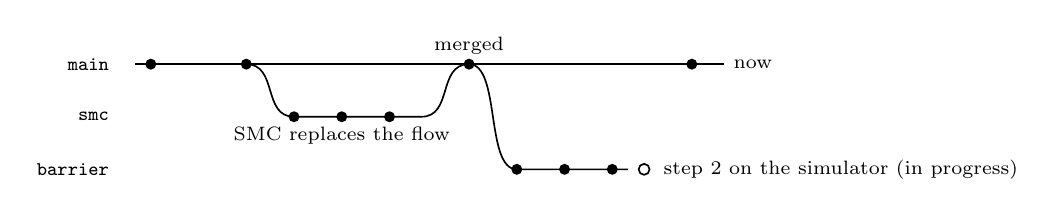
\begin{tikzpicture}[x=1.15em,y=1.9em,dot/.style={circle,fill,inner sep=1.4pt},font=\scriptsize]
\node[left] at (0,0) {\texttt{main}};
\node[left] at (0,-1) {\texttt{smc}};
\node[left] at (0,-2) {\texttt{barrier}};
\draw (0.5,0) -- (19,0);
\foreach \x in {1,4,11,18} \node[dot] at (\x,0) {};
\draw (4,0) .. controls (5,0) and (4.5,-1) .. (5.5,-1) -- (9.5,-1) .. controls (10.5,-1) and (10,0) .. (11,0);
\foreach \x in {5.5,7,8.5} \node[dot] at (\x,-1) {};
\draw (11,0) .. controls (12,0) and (11.5,-2) .. (12.5,-2) -- (16,-2);
\foreach \x in {12.5,14,15.5} \node[dot] at (\x,-2) {};
\node[draw,dot,fill=white] at (16.5,-2) {};
\node[below,align=center] at (7,-1) {SMC replaces the flow};
\node[right] at (16.8,-2) {step 2 on the simulator (in progress)};
\node[above] at (11,0) {merged};
\node[right] at (19,0) {now};
\end{tikzpicture}
\end{center}

\Sub{D.2 Symbols}
Chosen by you from Nerd Font glyphs, after \you{19 Oct}{want to overhaul almost all the symbols - we have nerd font glyphs}. Done and failed match kairos's task boxes, at your request. On screen, colour adds meaning on top of shape, staying within the theme colours \youx{19 Oct}.

\begin{center}
\begin{tabular}{@{}c l @{\qquad} c l @{\qquad} c l@{}}
\toprule
\g{F01A4} & attended & \g{F0E47} & needs you & \g{F1276} & decision: re-check \\
\g{F01A3} & unattended & \g{F0904} & idle & \g{F033E} & decision: holding \\
\g{F0178} & unread & \g{F0135} & done & \g{F00FB} & decision: re-decided \\
\g{F04E6} & working & \g{F0158} & failed & \g{F0B4E} & scout find \\
\midrule
\g{F1004} & reading & \g{F0D13} & ink & \g{F00ED} & calendar \\
\g{F0335} & idea & \g{F173E} & answer & \g{F01EE} & mail \\
\g{F062C} & commits & \g{F028C} & chat & \g{F0D39} & approve list \\
\g{F0219} & dossier & \g{F06A9} & automatic action & \g{F0756} & chores \\
\g{F14DF} & project & \g{F04C5} & budget & & \\
\bottomrule
\end{tabular}
\end{center}

\Sec{E. Background work and its budget}
\begin{itemize}
\item \textbf{Measured first.} Every job logs its tokens. One calibration run of a dossier build, an answer and an ink readback against \texttt{/usage} turns tokens into a share of your weekly limit.
\item \textbf{Cap} about 15\% of the week \agreed{16 Oct}. Heavy jobs run overnight. Nothing starts while your own use of the current 5-hour window is above about 60\% \youx{17 Oct}.
\item \textbf{When short}, jobs give way in this order: answers (never skipped), ink readback, change records, dossiers, scout, reading \youx{17 Oct}. Learning material you asked for ranks with answers, since you are waiting on it \prop; area briefs ride on change records and cost little.
\item \textbf{Models} \prop: Haiku for change records; Sonnet for ink readback, answers and the scout's searching; Opus for dossier builds and for choosing the scout's finds.
\item \textbf{Its own view}: the week against the cap, the 5-hour window, each day by job type, the most expensive jobs, and cost by project \youx{18 Oct}.
\end{itemize}

\clearpage
\Sec{F. Build order}

{\small\renewcommand{\arraystretch}{1.15}
\begin{tabularx}{\linewidth}{@{}l >{\hsize=1.3\hsize}Y >{\hsize=0.7\hsize}Y@{}}
\toprule
Slice & What & Done when \\
\midrule
0 & \textbf{Plumbing.} The local-to-GitHub-to-server flow; one HTTP service; LaTeX bug fixed; one-column even-margin preamble for every tablet document, and the explainer skill rewritten to match; push folders; daily page, recall and their nightly steps off; \textbf{why nothing has entered the library since 6 September, and the generic-word link filter on}; budget logging; kairos on the shared taxonomy; laptop transcripts syncing; secrets scrubber; passwords changed. & Tablet pushes and readback work with no hand steps, the library takes new documents again, and nothing old runs at night. \\
1 & \textbf{Every screen, on fixtures.} Paper rounds are done (two markups); now the ratatui prototype in your locus window, with your symbols and the branch graph, in rounds until you are happy. Contracts frozen per screen. & You would be glad to keep it open, with fake data. \\
2 & \textbf{The dossier loop.} Change records; one checked decision-log format in every repository, the CV repository registered; dossiers for nabla, then QUAST; ink readback, highlights included, through the 95\% gate; the writer agent. & Both dossiers build from one command, your ink comes back sorted and confirmed, and any chat can be sent to paper as an explainer. \\
3 & \textbf{Project view live.} Where you are, the branch graph, New, sessions via Claude Code hooks, ask line, Answered, Decisions; area briefs and \texttt{context()} \prop. & You use it during a real deep block, and a chat elsewhere pulls current context. \\
4 & \textbf{Home live.} Projects, approvals and the auto log, System, the rhythm grid; Jot. & Home replaces checking things by hand. \\
5 & \textbf{The linking job}, then \textbf{Explore and the scout}; reading; the weekly review with the orphan check. & Links appear only with a reason you agree with; a week of finds graded with reasons. \\
6 & \textbf{The learning system}: goals and topic tracks, interview prep as one part, practice sheets with marked answers, ``defend every bullet''. & One real goal (an interview, or the internship) run through it. \\
7 & Canvas, search over everything, the area chart, the budget view. & Each used within two weeks of landing, or cut (R9). \\
\bottomrule
\end{tabularx}}

\medskip
Day to day you see only what is live; each slice turns its screens on. The two-week working-mode trial starts when slice 3 is live.

\Sec{G. Still open}
\begin{itemize}
\item \textbf{In the prototype rounds:} how the Project view stops being a wall of text, the branch graph first (\you{19 Oct}{May need to tune this some more, not sure how}); the work section's visual (rhythm grid by default, area chart one key away, still to prove); keryx at the window size; whether New splits into kinds; a detail pane for Changes; the weekly review in use.
\item \textbf{Decided in their slice, from something real:} the scout's first briefs and starting taste; what Canvas pulls; how a learning goal becomes a syllabus; practice-sheet format.
\item \textbf{The research track} (decisions and their evidence as a dependency graph, so overturned evidence flags what rests on it) starts after the dossier loop works \agreed{16 Oct}, with a decision network to view \youx{19 Oct}.
\item \textbf{Anything else.} Write below anything you would use locus for, or worry about, that is not here.
\end{itemize}

\vspace{14em}

\end{document}
